\documentclass[a4paper,12pt,obeyspaces,spaces,hyphens]{article}

\def \trainingtitle{Formation optimisation du temps de démarrage de Linux embarqué}
\def \trainingtype{onsite}
\def \trainingduration{3}
\def \agendalanguage{french}
\def \training{boot-time}

\usepackage{agenda}

\begin{document}

\feshowtitle

\feagendasummaryitem{Titre}{
  {\bf \trainingtitle{}}
}
\feagendasummaryitem{Objectifs\newline opérationnels}{
  \begin{itemize}
  \item Être capable d'utiliser les outils et techniques pour mesurer
    le temps de démarrage d'un système embarqué.
  \item Être capable de réduire le temps de démarrage au niveau de
    l'initialisation de l'espace utilisateur Linux.
  \item Être capable de réduire le temps de démarrage au niveau de
    l'initialisation du noyau Linux.
  \item Être capable de réduire le temps de démarrage au niveau de
    l'initialisation du chargeur de démarrage.
  \item Être capable de mettre en oeuvre d'autres techniques avancées
    et alternatives d'optimisation du temps de démarrage.
  \end{itemize}
}
\feagendasummaryitem{Durée}{
  \feshowduration{}
}
\onsitepedagogics{40}{60}{boot-time}
\feagendasummaryitem{Formateur}{
  Un des ingénieurs mentionnés sur :
  \newline \url{https://bootlin.com/training/trainers/}
}
\feagendasummaryitem{Langue}{
  Présentations : Français
  \newline Supports : Anglais
}
\feagendasummaryitem{Public visé}{
  Sociétés et ingénieurs développeurs de systèmes Linux embarqués.
  \newline Personnes offrant de l'assistance à de tels développeurs.
}
\feagendasummaryitem{Pré-requis}{
  \begin{itemize}
    \prerequisitecommandline
    \prerequisiteembeddedlinux
    \prerequisiteenglish
  \end{itemize}
}
\feagendasummaryitem{Équipement nécessaire}{
  {\bf Pour les sessions sur site uniquement}
  \newline Le matériel est fourni par Bootlin durant les
  sessions inter-entreprises
  \begin{itemize}
  \item Projecteur vidéo
  \item Un ordinateur sur chaque bureau (pour une ou deux personnes), avec au
    moins 8 Go de RAM, un processeur au moins équivalent à un Intel Core i5,
    et Ubuntu Linux installé dans une {\bf partition
      dédiée d'au moins 40 Go. L'utilisation de Linux dans une machine virtuelle
      n'est pas supportée}, en raison de problèmes avec la connexion au matériel.
  \item Nous avons besoin d'Ubuntu Desktop 20.04 (Xubuntu et autres
    variantes fonctionnent également). Nous ne supportons pas d'autres
    distributions, car nous ne pouvons tester toutes les versions des
    paquets.
  \item {\bf Connexion à Internet} (directe ou par le proxy de l'entreprise).
  \item {\bf Les ordinateurs contenant des données importantes doivent être
      sauvegardés} avant d'être utilisés dans nos sessions. Certains
    participants ont déjà commis des erreurs lors de travaux pratiques
    avec pour conséquence des pertes de données.
  \end{itemize}
}
\certificate{}
\disabilities{}

\feagendatwocolumn
{Matériel}
{
  La plateforme matérielle utilisée pendant les travaux pratiques de
  cette formation est la carte {\bf BeagleBone Black}, dont voici les
  caractéristiques :

  \begin{itemize}
  \item Un processeur ARM AM335x de Texas Instruments (à base de
    Cortex-A8), avec accélération 3D, etc.
  \item 512 Mo de RAM
  \item 2 Go de stockage eMMC embarqué sur la carte
	\newline(4 Go avec la révision C)
  \item USB hôte et device
  \item Sortie HDMI
  \item Connecteurs à 2 x 46 broches, pour accéder aux UARTs, aux
        bus SPI, aux bus I2C, et à d'autres entrées/sorties du
        processeur.
  \end{itemize}
}
{}
{
  \begin{center}
    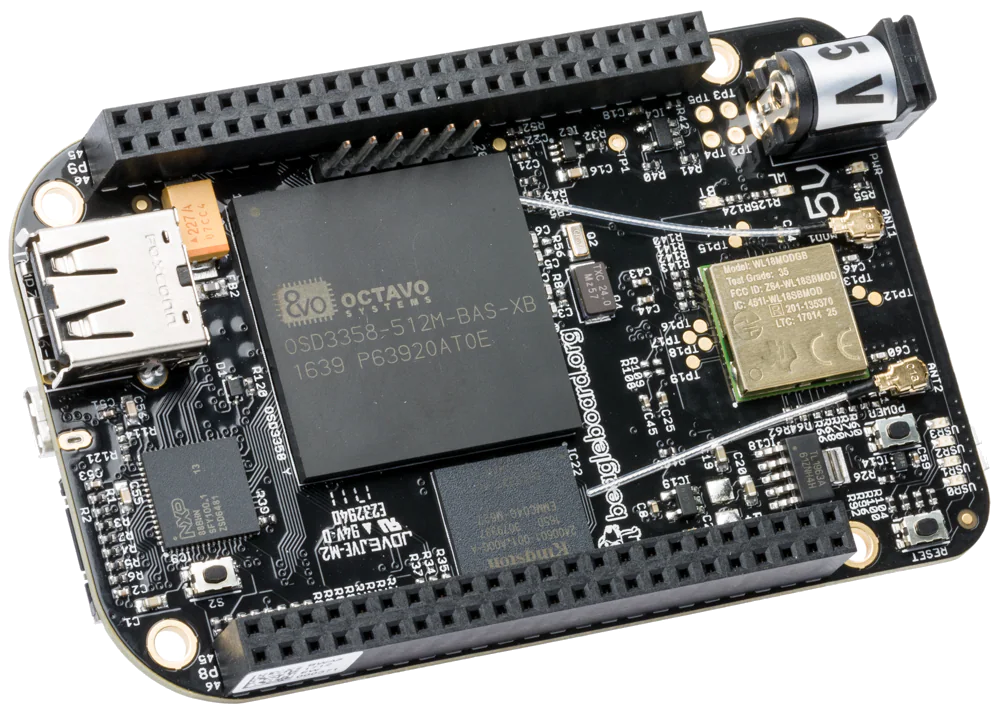
\includegraphics[height=5cm]{../slides/beagleboneblack-board/beagleboneblack.png}
  \end{center}
}

\feagendaonecolumn
{Démonstrations}
{
  Les démos de cette formation utiliseront les périphériques matériels suivants:

  \begin{itemize}
  \item Une webcam USB
  \item Une carte d'extension d'écran tactile LCD connectée à la carte
    BeagleBone Black, pour afficher la vidéo capturée par la webcam.
  \item Nous utiliserons également une carte Arduino comme moyen pour mesurer
    précisément le temps de démarrage, pour montrer comment mettre en place
    des techniques de mesure matérielles.
  \end{itemize}
}

\section{1\textsuperscript{er} jour - Matin}

\feagendatwocolumn
{Cours - Méthodes}
{
  \begin{itemize}
  \item Comment mesurer le temps de démarrage
  \item Principales approches
  \end{itemize}
}
{TP - Construction du système}
{
 \begin{itemize}
 \item Téléchargement du code source du chargeur de démarrage, du noyau et de Buildroot
 \item Prise en main de la carte, mise en place de la communication série
 \item Configuration de Buildroot et génération du système
 \item Configuration et compilation du chargeur de démarrage U-Boot. Préparation d'une
       carte SD pour démarrer le système.
 \item Configuration et compilation du noyau. Démarrage du système.
 \end{itemize}
}

\section{1\textsuperscript{er} Jour - Après-midi}

\feagendatwocolumn
{Cours - Mesure du temps}
{
  \begin{itemize}
  \item Techniques génériques par logiciel
  \item Techniques matérielles
  \item Solutions spécifiques à chaque étage du démarrage
  \end{itemize}
}
{TP - Mesure du temps - Solution logicielle}
{
 \begin{itemize}
 \item Modification du système pour mesurer le temps au niveau des différentes étapes.
 \item Chronométrer les messages sur la console série
 \item Chronométrer le démarrage de l'application
 \end{itemize}
}

\feagendatwocolumn
{TP - Mesure du temps - Solution matérielle}
{
  \begin{itemize}
  \item Mesure du temps total de démarrage en positionnant une GPIO
  \item Mise en oeuvre d'une carte Arduino
  \item Préparation d'un circuit de test avec un afficheur à 7 segments
  \item Modification du DTS pour configurer les broches de la Bone Black en tant que GPIOs
  \item Modification de l'application pour piloter les GPIOs personnalisées
  \end{itemize}
}
{Cours - Optimisations des chaînes de compilation}
{
  \begin{itemize}
  \item Introduction aux chaînes de compilation
  \item Bibliothèques C
  \item Informations de taille
  \item Mesure de la performance d'un exécutable avec la commande \code{time}
  \end{itemize}
}

\feagendaonecolumn
{TP - Optimisations des chaînes de compilation}
{
  \begin{itemize}
  \item Mesure du temps d'exécution de l'application
  \item Passage à une chaîne Thumb2
  \item Génération d'un SDK Buildroot pour recompiler plus vite
  \end{itemize}
}

\section{2\textsuperscript{ème} Jour - Matin}

\feagendatwocolumn
{Cours - Optimisation de l'application}
{
  \begin{itemize}
  \item Utilisation de \code{strace} et \code{ltrace}
  \item Autres techniques de profiling
  \end{itemize}
}
{TP - Optimisation de l'application}
{
 \begin{itemize}
 \item Rechercher d'options de configuration inutiles dans des applications
 \item Modification de ces options à travers Buildroot
 \item Expériences avec \code{strace} pour suivre l'exécution d'un programme
 \end{itemize}
}

\feagendatwocolumn
{Cours - Optimisation du démarrage du système}
{
  \begin{itemize}
  \item Utilisation de BusyBox \code{bootchartd}
  \item Optimisation des scripts d'init
  \item Possibilité de démarrer directement votre application
  \end{itemize}
}
{TP - Optimisation du démarrage du système}
{
 \begin{itemize}
 \item Utilisation de Buildroot pour supprimer scripts et commandes non nécessaires
 \item Une méthode pour identifier tous les fichiers inutilisés
 \item Simplification de BusyBox
 \item Démarrage de l'application en tant que programme init.
 \end{itemize}
}

\section{2\textsuperscript{ème} Jour - Après-midi}

\feagendatwocolumn
{Cours - Optimisations de systèmes de fichiers}
{
  \begin{itemize}
  \item Systèmes de fichiers disponibles, aspects de performance et de temps de démarrage
  \item Comment accélerer UBIFS
  \item Paramètres pour réduire le temps de démarrage
  \item Démarrer depuis un initramfs
  \item Utilisation d'exécutables statiques: contraintes de licence
  \end{itemize}
}
{TP - Optimisations de systèmes de fichiers}
{
 \begin{itemize}
 \item Essayer et mesurer deux systèmes de fichiers bloc: ext4 et SquashFS.
 \item Essai et benchmark de la solution initramfs. Contraintes
       en rapport avec cette solution.
 \end{itemize}
}

\feagendatwocolumn
{Cours - Optimisations du noyau}
{
  \begin{itemize}
  \item Utilisation d'{\em Initcall debug} to générer un {\em boot graph}
  \item Options de compression et liées à la taille
  \item Réduction ou suppression de la sortie console
  \item Plusieurs réglages pour réduire le temps de démarrage
  \end{itemize}
}
{TP - Optimisations du noyau}
{
 \begin{itemize}
 \item Génération et analyse d'un {\em boot graph} pour le noyau
 \item Identifier et éliminer les fonctionnalités du noyau non nécessaires
 \item Trouver la meilleure option de compression pour votre système
 \end{itemize}
}

\section{3\textsuperscript{ème} Jour - Matin}

\feagendaonecolumn
{TP - Optimisations du noyau}
{
 \begin{itemize}
 \item Poursuite du TP
 \end{itemize}
}

\section{3\textsuperscript{ème} Jour - Après-midi}

\feagendatwocolumn
{Cours - Optimisations du chargeur de démarrage}
{
  \begin{itemize}
  \item Conseils génériques pour réduire la taille et le temps
        de démarrage d'U-Boot.
  \item Optimisation des scripts d'U-Boot et du chargement du noyau
  \item Sauter le chargeur de démarrage - Comment modifier U-Boot pour
	activer son {\em Falcon mode}
  \end{itemize}
}
{Cours - Le {\em Falcon mode} d'U-Boot}
{
  \begin{itemize}
  \item Principes et objectifs
  \item Prétraîtement effectué par U-Boot pour préparer le démarrage de Linux
  \item Utilisation de la commande \code{spl export} pour faire ce traîtement à l'avance.
  \item Modification du code source d'U-Boot et configuration pour démarrer directement
        Linux et sauter le deuxième étage d'U-Boot.
  \item Exemples and instructions de mise en oeuvre sur MMC et flash NAND
  \item Comment débugger le Falcon mode
  \item Comment revenir à U-Boot
  \item Limitations
  \end{itemize}
}

\feagendaonecolumn
{TP - Optimisations du chargeur de démarrage}
{
 \begin{itemize}
 \item Utilisation des techniques ci-dessus pour rendre le chargeur
       de démarrage le plus rapide possible
 \item Passer à un stockage plus rapide
 \item Sauter le chargeur de démarrage avec le {\em Falcon mode} d'U-Boot
 \end{itemize}
}

\feagendaonecolumn
{Conclusion - Résultats obtenus}
{
 \begin{itemize}
 \item Partage et comparaison des résultats obtenus par les différents groupes
 \item Questions / réponses, partage d'expérience avec le formateur
 \end{itemize}
}

\end{document}
